\newcommand{\databaseName}{Elasticsearch}
\chapter{Implementation}\label{ch:implementation}


\section{Slurm}\label{subsec:slurm}

Slurm is an open-source management tool for Linux clusters \cite{slurm-online}.
It allocates recources, i.e. compute nodes, and provides the means to start, execute and monitor jobs \cite{slurm-online, slurm2003}.

The so-called slurm deamons control nodes, partitions, jobs and job steps \cite{slurm-online}.
According to \citeauthor{slurm-online}, a partition is a group of nodes and a job is the allocation of ressources, i.e. compute nodes, to an user for a limited time period.
A basic visualization of the architecture is given in \autoref{fig:slurm-architecture}.

\begin{figure}[htp] % htp = hier (h), top (t), oder auf einer eigenen Seite (p).
    \centering
    \includesvg[width=0.7\textwidth]{images/slurm_architecture}
    \caption{Slurm architecture. The management node has a \texttt{slurmctld} deamon, while every compute node has a \texttt{slurmd} deamon.
    The nodes communicate.
    The user can use certain commmands, for instance \texttt{srun} and \texttt{squeue}, anywhere on the cluster.
    }
    \label{fig:slurm-architecture}
\end{figure}

% Christians Skizzen der Verbindung(sherstellung)





\section{Database Elasticsearch}\label{subsec:db}
% introduction, users
\databaseName{} is a widely used non-relational database, which was designed to store and perform full-text search on large corpus of unstructured data \cite{Elasticsearch2017}.
This open-source distributed document-driven database system is build in Java and is based on the Apache Lucene (Java) library for high-speed full-text search \cite{Elasticsearch2017,Elasticsearch2019}.
According to \citeauthor{Elasticsearch2019}, \databaseName{} provides Wikipedia's full-text search and suggestions as well as Github's code search and Stack Overflow's geolocation queries and related questions.
It enables near real-time search by index refreshing periods of one second.
Needless to say, \databaseName{} is qualified to handle Big Data.

% structure
\databaseName{}'s entries, i.e. documents, are stored in logical units, so called indices.
% index
As stated by \citeauthor{Elasticsearch2019} and \citeauthor{Elasticsearch2017}, the indices are structured similar to Apache Lucene's inverted index format.
An index can be spread into multiple nodes.
A node is single running instance of \databaseName{} \cite{Elasticsearch2019}.
An index is divided into one or more shards, which can be stored on different servers and enable parallelization \cite{Elasticsearch2019}.

% document
\databaseName{} indices' entries are documents, which are saved in a \ac{json} fromat \cite{Elasticsearch2017}.
A document's fields and field types are defined by the user when initializing the database index.
By default, every field of a document is indexed and searchable \cite{Elasticsearch2019}.

% Replicas
Replicas are copies of shards, which create redundancy and thus, ensure availability \cite{Elasticsearch2019}.

% content
The database is filled once with data from a large unstructured corpus of \ac{pdf} files.
After the initialization of the database, it is used for queries. 
Therefore, the workflow is completely offline.

The index \textit{Bahamas} stores different embeddings of the text layer information and metadata of the documents.
As depicted in \autoref{fig:pdf2db}, not only textual information is stored in the database, but also the images of the first page of the \acp{pdf}.
The structure of the index is presented in \autoref{tbl:Elasticsearch-fields}.

% TODO: add field type or dimension?
\begin{table}[]
    \caption{Fields in \databaseName{} database in index \textit{Bahamas}.}
    \begin{tabular}{|
    >{\columncolor[HTML]{EFEFEF}}l |p{0.63\textwidth}|}
    \hline
    \cellcolor[HTML]{C0C0C0}\textbf{field name} & \cellcolor[HTML]{C0C0C0}\textbf{field description}                                     \\ \hline
    \_id                                        & Unique identifier of document \texttt{i}. The identifier is generated by the sha256 hash algorithm from hashlib.\\ \hline
    doc2vec                                     & 55 dimensional doc2vec embedding of \texttt{i}.                                                          \\ \hline
    sim\_docs\_tfidf                            & sim\_docs\_tfidf embedding + all-zero flag of \texttt{i}. The all-zero flag is one, if the \ac{tfidf} embedding consists of only zeros, zero else.\\ \hline
    google\_univ\_sent\_encoding                & 512 dimensional google\_univ\_sent\_encoding embedding of \texttt{i}.                                     \\ \hline
    huggingface\_sent\_transformer              & 384 dimensional huggingface\_sent\_transformer embedding of \texttt{i}.                                  \\ \hline
    inferSent\_AE                               & inferSent\_AE embedding of \texttt{i}. Since the pretrained infersent model embedding's dimension is 4096, the encoder of a trained \ac{ae} is added to reduce the dimension to 2048.                                                    \\ \hline
    pca\_image                                  & Two dimensional \ac{pca} version of first page image of \texttt{i}.                      \\ \hline
    pca\_kmeans\_cluster                        & Cluster of \texttt{i} identified by KMeans on \ac{pca} version of image.                 \\ \hline
    text                                        & Text of \texttt{i}.                                                                       \\ \hline
    path                                        & Path on local maschine to \texttt{i}.                                                     \\ \hline
    image                                       & Base64 encoded image of first page of \texttt{i}.                                                        \\ \hline
    \end{tabular}
    \label{tbl:Elasticsearch-fields}
\end{table}

\begin{figure}[htp] % htp = hier (h), top (t), oder auf einer eigenen Seite (p).
    \centering
    \includesvg[width=0.7\textwidth]{images/PDFs_to_database}
    \caption{\acp{pdf} to Database. 
    First, the data is preprocessed:
    The first page of a \ac{pdf} file is converted to an image and the complete text is extracted. 
    The images are stored in the database as well as the text and different embeddings of the text.
    }
    \label{fig:pdf2db}
\end{figure}

% query (endpoints)
% get: search id
By specifying the unique \texttt{\_id} of a document and the database \texttt{index}, it is possible to retrieve a specific document from the database using the \texttt{GET \ac{api}}.
The query is real-time by default.
The parameters \texttt{\_source\_excludes} or \texttt{\_source\_includes} may be used to exclude or include specific fields of the document in the response \cite{Elasticsearch-get}.

% full-text search
The keyword used when performing full-text search is \texttt{match}.
To query for a specific value, one has to specify the \texttt{<field>} of interest and the query value.

\databaseName{} preprocesses the query value before starting the search \cite{Elasticsearch-text-analyser}.
The default preprocessing steps of the so-called default analyser include tokenization and lowercasing \cite{Elasticsearch-standard-analyser}. 
Omitting stop words is disabled by default, but it is possible to provide custom stop words or use the English stop word list \cite{Elasticsearch-standard-analyser}.
It is possible to create custom tokenizers, which split the query value into tokens of a certain maximum length.
In this work, the default analyser is used for the full-text search, since for instance configuring a maximum token length did not seem necessary or likely to improve the results.

Another useful feature of \databaseName{} is the multi-terms synonym expansion.
When the user queries a specific phrase \databaseName{} expands the query to include synonyms of the query terms \cite{Elasticsearch-synonyms}.
The maximum number of expansion terms is set to 50 by default, but can be configured by the user \cite{Elasticsearch-match}.
By default, the multi-terms synonym expansion option is enabled \cite{Elasticsearch-match}.

\databaseName{} also provides the option to perform fuzzy matching instead of exact search.
By enabling the fuzzy matching option, a \databaseName{} query consisting of for instance, \textit{Bahama} returns documents which have the word \textit{Bahamas}.
By default this option is not enabled, but can be enabled and configured individually by the user \cite{Elasticsearch-match}.
In this work, the fuzzy matching option is set to \texttt{AUTO}, which means in terms of keyword or text fields that the allowed Levenshtein Edit Distance, 
i.e. number of characters changed to create an exact match between two terms, to be considered a match, is correlated to the length of the term \cite{Elasticsearch-fuzziness}.
By default, terms of length up to two characters must match exactly, terms of length three to five characters must have an edit distance of one and 
terms of length six or more characters must have an edit distance of two \cite{Elasticsearch-fuzziness}.

% knn-search
Another search option of \databaseName{} is the \ac{knn} search.
The return value of a \ac{knn} search are the \texttt{k} nearest neighbors in terms of a certain distance function of a query vector \cite{Elasticsearch-kNN-HNSW}.
According to \citeauthor{Elasticsearch-kNN-HNSW}, one of \ac{knn} search's use cases is semantic document retrieval, which makes it a good fit for this task.
The query is a dense vector of the same dimension as the (dense) vectors stored in the database.
According to \cite{Elasticsearch-knn}, the \ac{knn} either returns the exact brute-force nearest neighbors or approximate nearest neighbors calculated by the \ac{hnsw} algorithm \cite{Elasticsearch-kNN-HNSW, Elasticsearch-knn}.
In this work, the approximate nearest neighbors search is used, since it is faster and the results are good enough for the use case of this work.
\ac{hnsw} is a graph-based algorithm \cite{Elasticsearch-kNN-HNSW}.
The term \texttt{navigable} refers to the graphs used, which are graphs with (poly-)logarithmic scaling of links traversed during greedy traversal with respect to the network size \cite{Elasticsearch-kNN-HNSW}.
The idea of a \texttt{hiercharical} algorithm is to create a multilayer graph, grouping links according to their link length, as displayed in \autoref{fig:hnsw-layer}. 
The search starts on the uppermost layer, i.e. the layer containing the longest links, greedily traversing the layer until reaching the local minimum.
It uses this local minimum as the starting point at the next lower layer and the process is repeated until the lowest layer is reached \cite{Elasticsearch-kNN-HNSW}.
The layers of the graph are built incrementally, and a neighbour selection heuristic, as depicted in \autoref{fig:hnsw-heuristic}, not only creates links between close elements, 
but also between isolated clusters to ensure global connectivity \cite{Elasticsearch-kNN-HNSW}.

\begin{figure}[htp] % htp = hier (h), top (t), oder auf einer eigenen Seite (p).
    \centering
    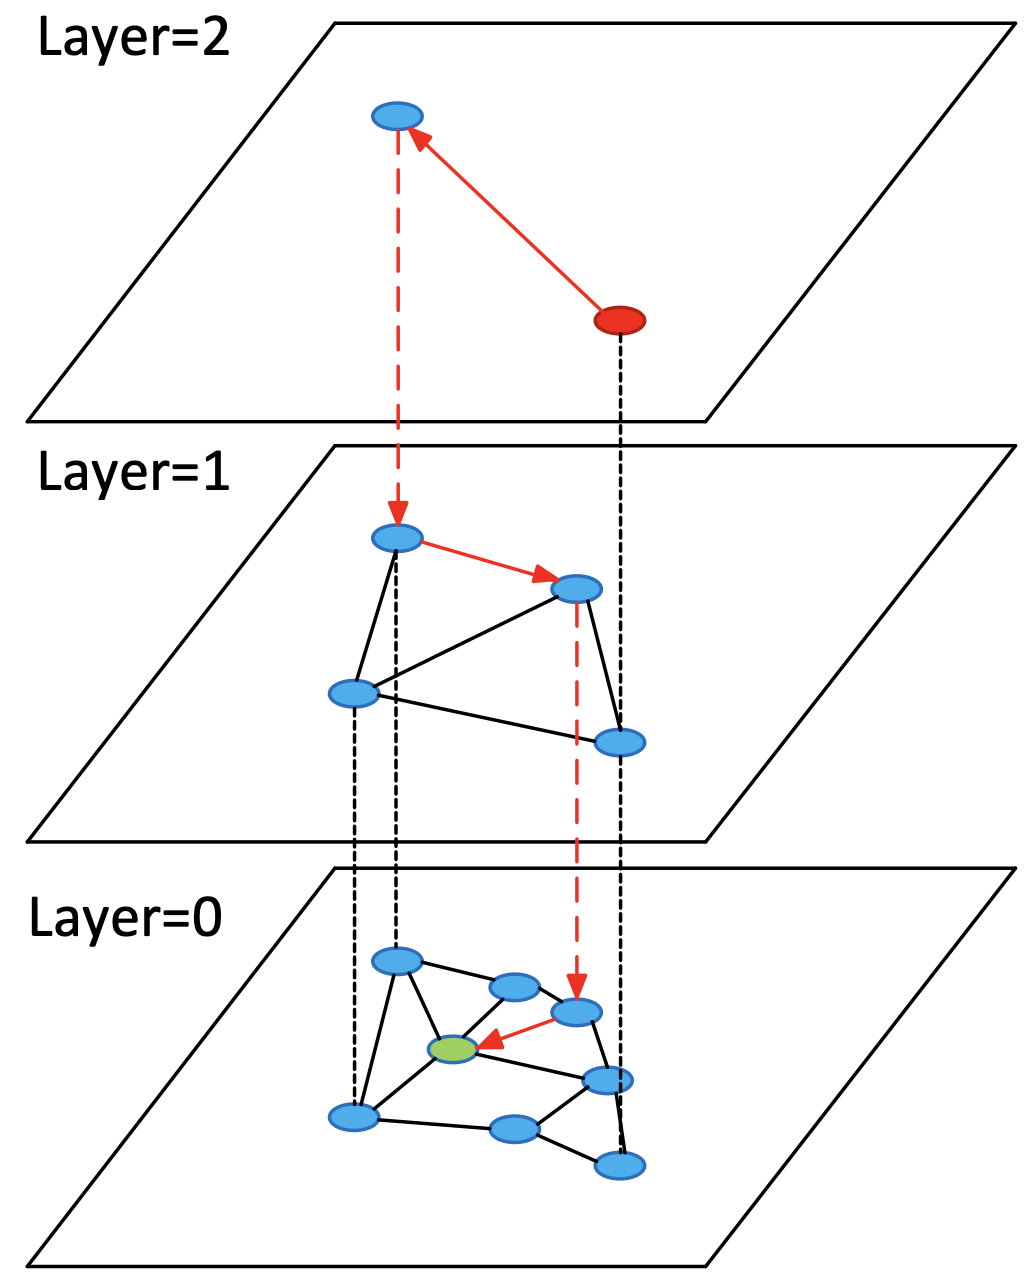
\includegraphics[width=0.3\textwidth]{images/HNSW-layer.png}
    \caption{Structure of \ac{hnsw} layer from \cite{Elasticsearch-kNN-HNSW}.
    The search starts on the uppermost layer, i.e. the layer containing the longest links, greedily traversing the layer until reaching the local minimum.
    The local minimum is used as the starting point at the next lower layer and the process is repeated until the lowest layer is reached.
    }
    \label{fig:hnsw-layer}
\end{figure}

\begin{figure}[htp] % htp = hier (h), top (t), oder auf einer eigenen Seite (p).
    \centering
    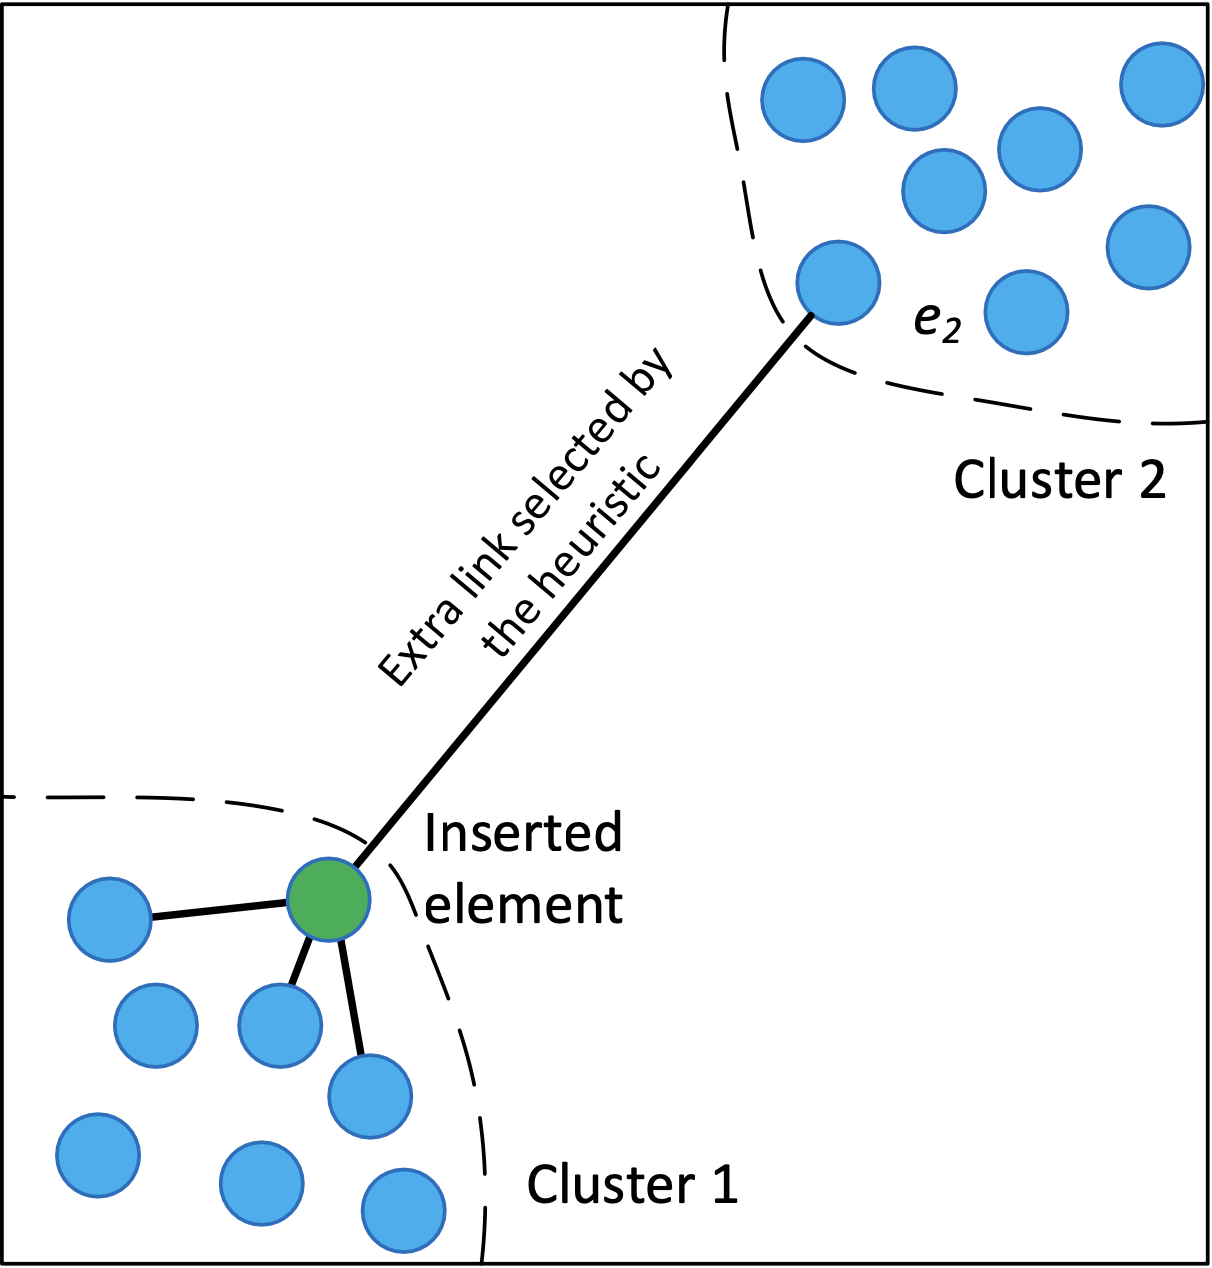
\includegraphics[width=0.3\textwidth]{images/HNSW-neighbour-selection-heuristic.png}
    \caption{Neighbour selection heuristic of \ac{hnsw} from \cite{Elasticsearch-kNN-HNSW}.
    The heuristic creates diverse links, i.e. links between close elements (e.g., green circle and elements in cluster 1) 
    and between isolated clusters (e.g., green circle and $e_2$) to ensure global connectivity.
    }
    \label{fig:hnsw-heuristic}
\end{figure}

In order to perform the \ac{knn} search on a \texttt{<field>} it has to be of type \texttt{dense\_vector}, indexed and a \texttt{similarity} measure has to be defined when initializing the database \cite{Elasticsearch-knn}.
The similarity measure used in this work is the cosine similarity, which calculates the \texttt{\_score} of a document according to \autoref{eq:cosine-similarity} from \cite{Elasticsearch-kNN-similarity}, 
where \texttt{query} is the query vector and \texttt{vector} is the vector representation of the document in the database.
Since cosine is not defined on vectors with zero magnitude, embeddings which can possibly return all zero vector representations, such as sim\_docs\_tfidf, are enhanced with an all-zero flag in this work.
\begin{equation}
    \frac{1 + \text{cosine}(\text{query}, \text{vector})}{2}
    \label{eq:cosine-similarity}
\end{equation}

\databaseName{}'s \ac{knn} implementation not only allows literal matching on search terms, but also semantic search \cite{Elasticsearch-knn}.
Besides \databaseName{}, the elastic stack offers other tools, for instance Kibana, which provides a user interface to manage different models.
After saving a model in Kibana, it is possible to create a text embedding ingest pipeline, which embeds new documents or reindexes existing documents \cite{Elasticsearch-knn-embedding}.
However, in this work, Kibana is not used and the used models are saved on disk as \ac{pkl} files.
Therefore, instead of using the \ac{knn} query structure for semantic search on embeddings provided by \databaseName{}, the normal \ac{knn} search on a field which contains an embedding is used.


\section{User Interface}\label{sec:ui}

\subsection{Backend}\label{subsec:backend}
Flask

\subsection{Frontend}\label{subsec:frontend}
angular